\lab{Pandas 2: Plotting}{Pandas 2: Plotting}
\objective{Clear, insightful visualizations are a crucial part of data analysis.
To facilitate quick data visualization, pandas includes several tools that wrap around matplotlib.
These tools make it easy to compare different parts of a data set, explore the data as a whole, and spot patterns and correlations in the data.}


% \begin{info}
% This lab will be done using Colab Notebooks.
% These notebooks are similar to Jupyter Notebooks but run remotely on Google's servers.
% Open a Google Colab notebook by going to your Google Drive account and creating a new Colaboratory file.
% If making a Colaboratory file is not an option, download the application Colaboratory onto your Google Drive.
% Once opening a new Colab Notebook, upload the file \li{pandas2.ipynb}.
% To make the data files accessible, run the following at the top of the lab:
% \begin{lstlisting}
% >>> from google.colab import files

% >>> uploaded = files.upload()
% \end{lstlisting}
% This will prompt you upload files for this notebook.
% For this lab, upload \li{crime_data.csv} and \li{college.csv}.

% Once the lab is complete, delete BOTH lines of code used for uploading files (the import statement and the upload statement) and download as a \li{.py} file to your git repository.
% Push the newly made \li{pandas2.py} file.
% \end{info}


\section*{Overview of Plotting Tools} % =======================================

The main tool for visualization in pandas is the \li{plot()} method for \li{Series} and \li{DataFrames}.
The method has a keyword argument \li{kind} that specifies the type of plot to draw.
The valid options for \li{kind} are detailed below.

\begin{table}[H]
\begin{tabular}{r|c|l}
Plot Type & \li{plot()} ID & Uses and Advantages \\ \hline
Line plot & \li{"line"} & Show trends ordered in data; easy to compare multiple data sets \\
Scatter plot & \li{"scatter"} & Compare exactly two data sets, independent of ordering \\
Bar plot & \li{"bar"}, \li{"barh"} & Compare categorical or sequential data \\
Histogram & \li{"hist"} & Show frequencies of one set of values, independent of ordering \\
% Kernel Density Estimation & \li{"kde"} & Estimate a smooth distribution \\
Box plot & \li{"box"} & Display min, median, max, and quartiles; compare data distributions \\
Hexbin plot & \li{"hexbin"} & 2D histogram; reveal density of cluttered scatter plots \\
\end{tabular}
\caption{Types of plots in pandas.
The plot ID is the value of the keyword argument \li{kind}.
That is, \li{df.plot(kind="scatter")} creates a scatter plot.
The default \li{kind} is \li{"line"}.}
\label{table:pandas-plot-options}
\end{table}

The \li{plot()} method calls \li{plt.plot()}, \li{plt.hist()}, \li{plt.scatter()}, and other matplotlib plotting functions, but it also assigns axis labels, tick marks, legends, and a few other things based on the index and the data.
Most calls to \li{plot()} specify the \li{kind} of plot and which \li{Series} to use as the \li{x} and \li{y} axes.
By default, the \li{index} of the \li{Series} or \li{DataFrame} is used for the \li{x} axis.

% In Pandas, a \li{DataFrame} is an ordered collection of \li{Series}.
% A Series is similar to a dictionary, with values assigned to various labels, or indices.
% Each Series becomes a column in the data frame, with each row corresponding to an index.
% When several Series are combined into a single data frame, it becomes very easy to compare and visualize data.
% Each entry has an associated index and column.

\begin{lstlisting}
>>> import pandas as pd
>>> from matplotlib import pyplot as plt

>>> budget = pd.read_csv("budget.csv", index_col="Date")
>>> budget.plot(y="Rent")  # Plot rent against the index (date).
\end{lstlisting}

\begin{figure}[H]
\centering
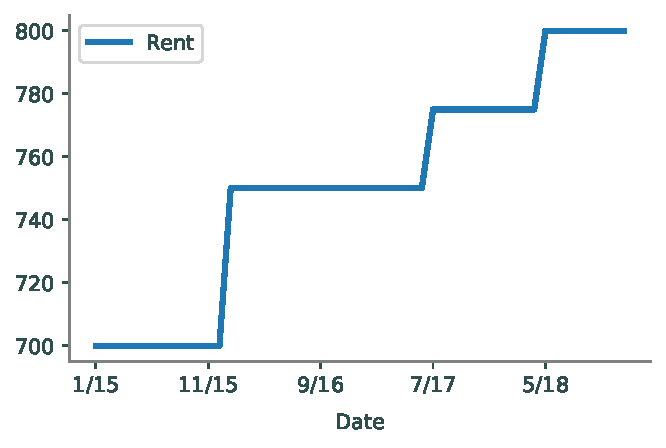
\includegraphics[width=.7\textwidth]{figures/Rent.pdf}
\end{figure}

In this case, the call to the \li{plot()} method is essentially equivalent to the following code.

\begin{lstlisting}
>>> plt.plot(budget.index, budget['Rent'], label='Rent')
>>> plt.xlabel(budget.index.name)
>>> plt.xlim(min(budget.index), max(budget.index))
>>> plt.legend(loc='best')
\end{lstlisting}

The \li{plot()} method also takes in many keyword arguments for matplotlib plotting and annotation functions.
For example, setting \li{legend=False} disables the legend, providing a value for \li{title} sets the figure title, \li{grid=True} turns a grid on, and so on.
For more customizations, see \url{https://pandas.pydata.org/pandas-docs/stable/generated/pandas.DataFrame.plot.html}.

\subsection*{Visualizing an Entire Data Set} % --------------------------------

A good way to start analyzing an unfamiliar data set is to visualize as much of the data as possible to determine which parts are most important or interesting.
For example, since the columns in a \li{DataFrame} share the same index, the columns can all be graphed together using the index as the $x$-axis.
By default, the \li{plot()} method attempts to plot \textbf{every} \li{Series} (column) in a \li{DataFrame}.
This is especially useful with sequential data, like the budget data set.

\begin{lstlisting}
# Plot all columns together against the index.
>>> budget.plot(title="All Budgets",linewidth=1)
>>> budget.drop(["Rent"], axis=1).plot(linewidth=1,title="All Budgets Except Rent")
\end{lstlisting}

\begin{figure}[H] % Plot everything together.
\captionsetup[subfigure]{justification=centering}
\centering
\begin{subfigure}{.49\textwidth}
    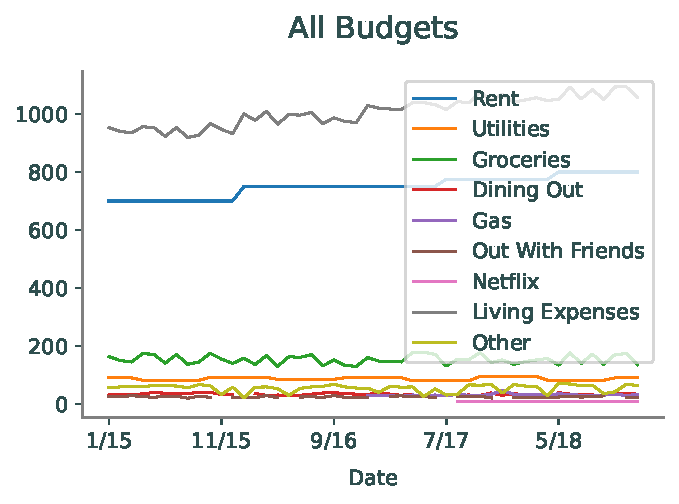
\includegraphics[width=\textwidth]{figures/all_budget.pdf}
    \caption{All columns of the budget data set on the same figure, using the index as the $x$-axis.}
    \label{fig:budget-all}
\end{subfigure}
%
\begin{subfigure}{.49\textwidth}
    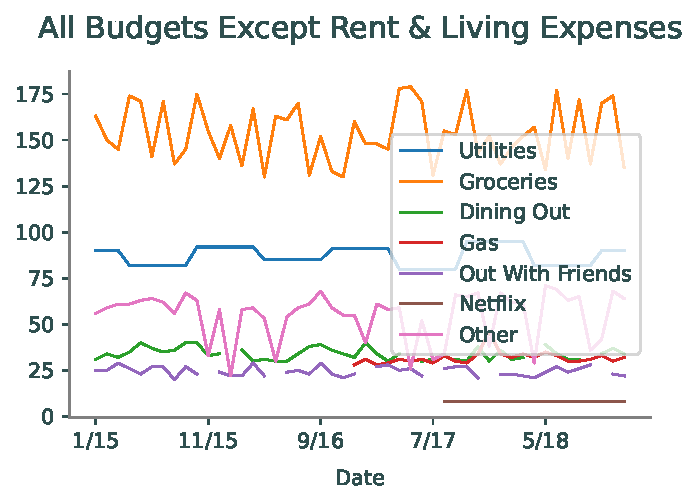
\includegraphics[width=\textwidth]{figures/all_budget2.pdf}
    \caption{All columns of the budget data set except \li{"Living Expenses"} and \li{"Rent"}.}
    \label{fig:budget-all-v2}
\end{subfigure}
\caption{}
\end{figure}

While plotting every \li{Series} at once can give an overview of all the data, the resulting plot is often difficult for the reader to understand.
For example, the budget data set has 9 columns, so the resulting figure, Figure \ref{fig:budget-all}, is fairly cluttered.

One way to declutter a visualization is to examine less data.
For example, the columns \li{'Living Expenses'} and \li{'Rent'} have values that are much larger than the other columns.
Dropping these columns gives a better overview of the remaining data, as shown in Figure \ref{fig:budget-all-v2}.

\begin{warn}
Often plotting all data at once is unwise because columns have \textbf{different units of measure}.
Be careful not to plot parts of a data set together if those parts do not have the same units or are otherwise incomparable.
\end{warn}

Another way to declutter a plot is to use subplots.
To quickly plot several columns in separate subplots, use \li{subplots=True} and specify a shape tuple as the \li{layout} for the plots.
Subplots automatically share the same $x$-axis.
Set \li{sharey=True} to force them to share the same $y$-axis as well.

\begin{lstlisting}
>>> budget.plot(y=['Dining Out','Gas','Out With Friends', 'Netflix'],
... 	subplots=True, layout=(2,2), sharey=True,
... 	style=['-','--','-.',':'],title="Plots of Dollars Spent for Different Budgets")
\end{lstlisting}

\begin{figure}[H]
    \includegraphics[width=.8\textwidth]{figures/line_subplots.pdf}
\end{figure}

As mentioned previously, the \li{plot()} method can be used to plot different kinds of plots.
One possible kind of plot is a histogram.
Since plots made by the \li{plot()} method share an $x$-axis by default, histograms turn out poorly whenever there are columns with very different data ranges or when more than one column is plotted at once.

\begin{lstlisting}
# Plot three histograms together.
>>> budget.plot(kind='hist',y=['Gas','Dining Out','Out With Friends'],
... 	alpha=.7,bins=10,title="Frequency of Amount (in dollars) Spent")

# Plot three histograms, stacking one on top of the other.
>>> budget.plot(kind='hist',y=['Gas','Dining Out','Out With Friends'],
...		bins=10,stacked=True,title="Frequency of Amount (in dollars) Spent")
\end{lstlisting}

\begin{figure}[H] % Try to compare histograms.
\centering
\begin{subfigure}{.49\textwidth}
    \includegraphics[width=\textwidth]{figures/bad_hist_unstacked.pdf}
\end{subfigure}
%
\begin{subfigure}{.49\textwidth}
    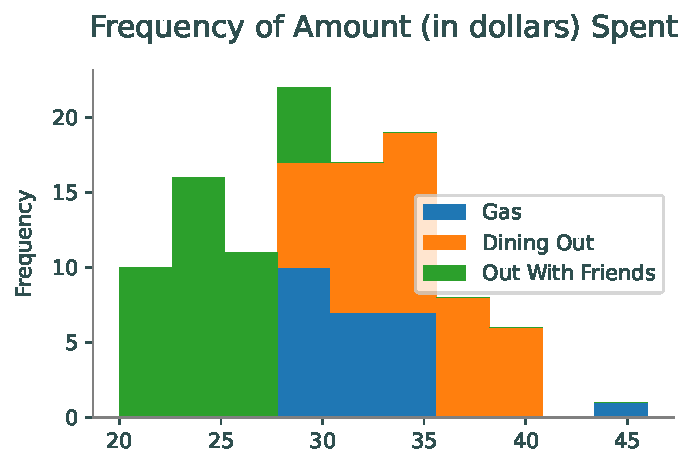
\includegraphics[width=\textwidth]{figures/bad_hist_stacked.pdf}
\end{subfigure}
\caption{Two examples of histograms that are difficult to understand because multiple columns are plotted.}
\end{figure}

Thus, histograms are good for examining the distribution of a \textbf{single} column in a data set.
For histograms, use the \li{hist()} method of the \li{DataFrame} instead of the \li{plot()} method.
Specify the number of bins with the \li{bins} parameter.
Choose a number of bins that accurately represents the data; the wrong number of bins can create a misleading or uninformative visualization.


\begin{lstlisting}
>>> budget[["Dining Out","Gas"]].hist(grid=False,bins=10)
\end{lstlisting}

\begin{figure}[H]
    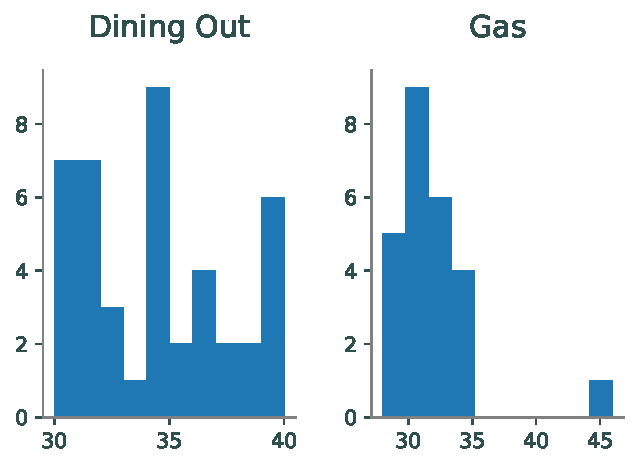
\includegraphics[width=.7\textwidth]{figures/hist_subplots.pdf}
   \caption{Histograms of \li{"Dining Out"} and \li{"Gas"}.}
\end{figure}

% Problem 1
\begin{problem}
Create 3 visualizations for the data in \li{crime_data.csv}.
Make one of the visualizations a histogram.
The visualizations should be well labeled and easy to understand.
%Include a short description of your plots as a caption.
\label{prob:hist}
\end{problem}

\section*{Patterns and Correlations} % ========================================

After visualizing the entire data set initially, a good next step is to closely compare related parts of the data.
This can be done with different types of visualizations.
For example, Figure \ref{fig:budget-all-v2} suggests that the \li{"Dining Out"} and \li{"Out With Friends"} columns are roughly on the same scale.
Since this data is sequential (indexed by time), start by plotting these two columns against the index.
Next, create a scatter plot of one of the columns versus the other to investigate correlations that are independent of the index.
Unlike other types of plots, using \li{kind="scatter"} requires both \li{x} and \li{y} columns as arguments.

\begin{lstlisting}

# Plot 'Dining Out' and 'Out With Friends' as lines against the index.
>>> budget.plot(y=["Dining Out", "Out With Friends"],title="Amount Spent on Dining Out and Out with Friends per Day")

# Make a scatter plot of 'Dining Out' against 'Out With Friends'
>>> budget.plot(kind="scatter", x="Dining Out", y="Out With Friends",
... 	alpha=.8,xlim=(0,max(budget['Dining Out'])+1),
...		ylim=(0,max(budget['Out With Friends'])+1))
\end{lstlisting}

\begin{figure}[H] 
\captionsetup[subfigure]{justification=centering}
\centering
\begin{subfigure}{.49\textwidth}
    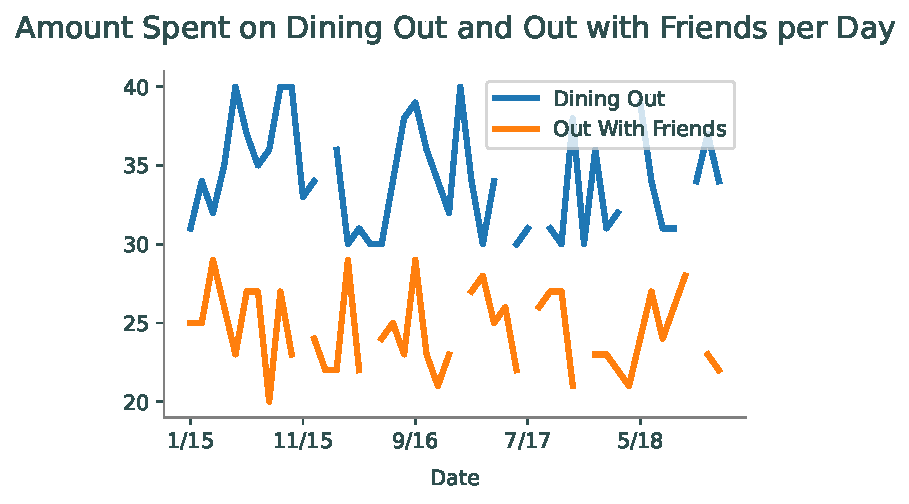
\includegraphics[width=\textwidth]{figures/line_compare.pdf}
\end{subfigure}
%
\begin{subfigure}{.49\textwidth}
    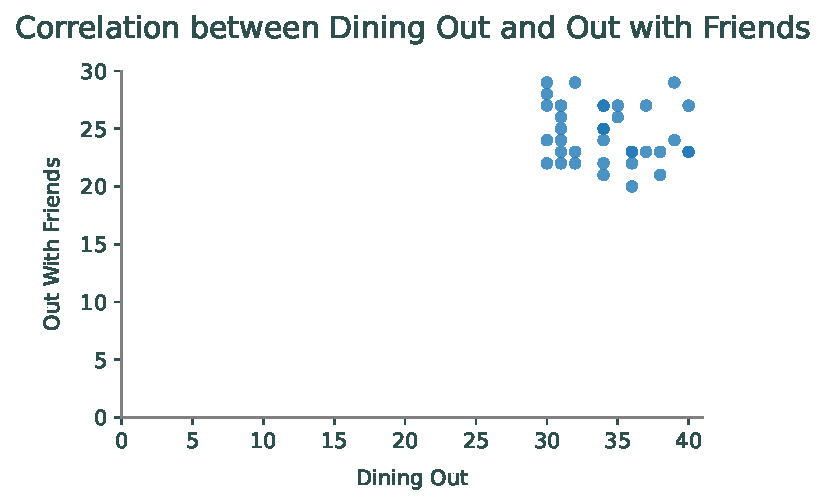
\includegraphics[width=\textwidth]{figures/scatter_compare.pdf}
\end{subfigure}
\caption{Correlations between \li{"Dining Out"} and \li{"Out With Friends"}.}
\end{figure}

The first plot shows us that more money is spent on dining out than being out with friends overall.
However, both categories stay in the same range for most of the data.
This is confirmed in the scatter plot by the block in the upper right corner, indicating the common range spent on dining out and being out with friends.

\begin{warn}
When analyzing data, especially while searching for patterns and correlations, \textbf{always} ask yourself if the data makes sense and is trustworthy.
What lurking variables could have influenced the data measurements as they were being gathered?

The crime data set from Problem \ref{prob:hist} is somewhat suspect in this regard.
The murder rate is likely accurate, since murder is conspicuous and highly reported, but what about the rape rate?
Are the number of rapes increasing, or is the percentage of rapes being reported increasing?
It's probably both!
Be careful about drawing conclusions for sensitive or questionable data.
\end{warn}

Another useful visualization used to understand correlations in a data set is a scatter matrix.
The function \li{pd.plotting.scatter_matrix()} produces a table of plots where each column is plotted against each other column in separate scatter plots.
The plots on the diagonal, instead of plotting a column against itself, displays a histogram of that column.
This provides a very quick method for an initial analysis of the correlation between different columns.

\begin{lstlisting}
>>> pd.plotting.scatter_matrix(budget[['Living Expenses','Other']])
\end{lstlisting}

\begin{figure}[H]
    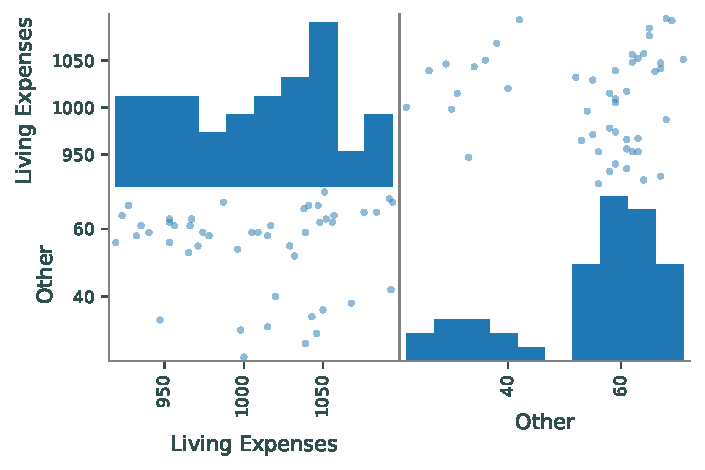
\includegraphics[width=.7\textwidth]{figures/scatter_table.pdf}
    \caption{Scatter matrix comparing \li{"Living Expenses"} and \li{"Other"}.}
\end{figure}


\subsection*{Bar Graphs}

Different types of graphs help to identify different patterns.
Note that the data set \li{budget} gives monthly expenses.
It may be beneficial to look at one specific month.
Bar graphs are a good way to compare small portions of the data set.

As a general rule, horizontal bar charts (\li{kind="barh"}) are better than the default vertical bar charts (\li{kind="bar"}) because most humans can detect horizontal differences more easily than vertical differences.
If the labels are too long to fit on a normal figure, use \li{plt.tight_layout()} to adjust the plot boundaries to fit the labels in.

\begin{lstlisting}
# Plot all data for the last month in the budget
>>> budget.iloc[-1,:].plot(kind='barh')
>>> plt.tight_layout()

# Plot all data for the last month without 'Rent' and 'Living Expenses'
>>> budget.drop(['Rent','Living Expenses'],axis=1).iloc[-1,:].plot(kind='barh')
>>> plt.tight_layout()
\end{lstlisting}

\begin{figure}[H] % Plot the early 1980s and the last year.
\captionsetup[subfigure]{justification=centering}
\centering
\begin{subfigure}{.49\textwidth}
    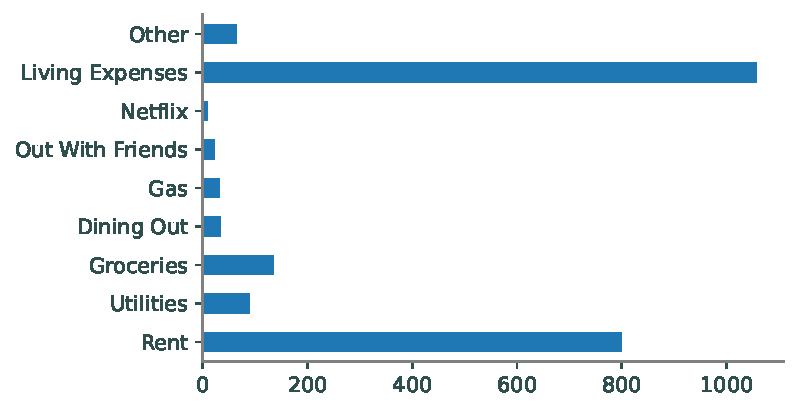
\includegraphics[width=\textwidth]{figures/all_expenses.pdf}
\end{subfigure}
%
\begin{subfigure}{.49\textwidth}
    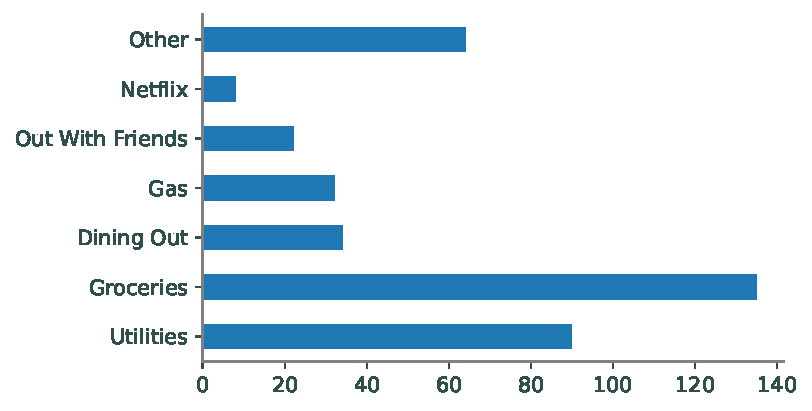
\includegraphics[width=\textwidth]{figures/some_expenses.pdf}
\end{subfigure}
\caption{Bar graphs showing expenses paid in the last month of \li{budget}.}
\end{figure}

% Problem 2
\begin{problem}
Using the crime data from the previous problem, identify if a trend exists between \li{Forcible Rape} and the following variables:
\begin{enumerate}
\item \li{Violent}
\item \li{Burglary}
\item \li{Aggravated Assault}
\end{enumerate}

Make sure each graph is clearly labelled and readable.
Return a tuple of booleans describing whether \li{Forcible Rape} correlates with each of the other variables.
\end{problem}

\section*{Distributional Visualizations} % ====================================

While histograms are good at displaying the distributions for one column, a different visualization is needed to show the distribution of an entire set.
A \emph{box plot}, sometimes called a ``cat-and-whisker'' plot, shows the five number summary: the minimum, first quartile, median, third quartile, and maximum of the data.
Box plots are useful for comparing the distributions of relatable data.
However, box plots are a basic summary, meaning that they are susceptible to  miss important information such as how many points were in each distribution.

\begin{lstlisting}

# Compare the distributions of four columns.
>>> budget.plot(kind="box", y=["Gas","Dining Out","Out With Friends","Other"])

# Compare the distributions of all columns but 'Rent' and 'Living Expenses'.
>>> budget.drop(["Rent", "Living Expenses"], axis=1).plot(kind="box",
...		vert=False)
\end{lstlisting}

\begin{figure}[H] % Use box plots to compare distributions.
\captionsetup[subfigure]{justification=centering}
\centering
\begin{subfigure}{.49\textwidth}
    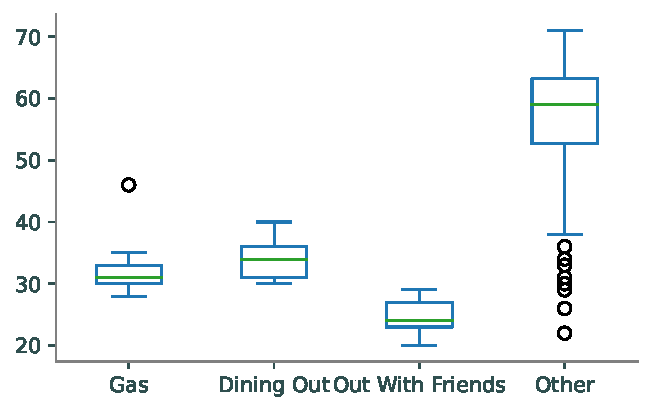
\includegraphics[width=\textwidth]{figures/box1.pdf}
\end{subfigure}
%
\begin{subfigure}{.49\textwidth}
    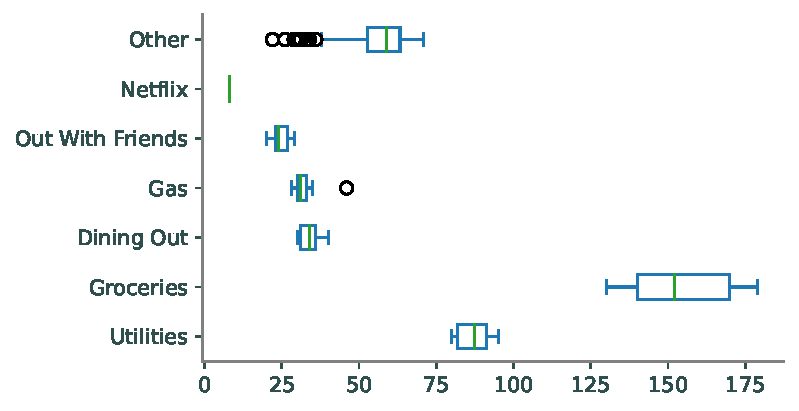
\includegraphics[width=\textwidth]{figures/box2.pdf}
\end{subfigure}
\caption{Vertical and horizontal box plots of \li{budget} dataset.}
\end{figure}

% TODO: KDE plot?

% TODO: hexbin plots

% Bar plots, on the other hand, are particularly useful for comparing several categories of data over time, or whenever there is a sense of progression in the index.
% Line plots are better suited to show a more continuous index (such as each year in a century), whereas bar plots are better for a discrete index (a few distinct years).
% Line and bar plots work well when there is a logical progression in the index, such as time.
% However, when frequency of occurrence is more important than the location of the data, histograms and box plots can be more informative.
% Use \li{plot(kind="hist")} to produce a histogram.
% Standard histogram options, such as the number of bins, are also accepted as keyword arguments.
% The \li{alpha} keyword argument makes each bin slightly transparent.

% Sometimes it is helpful to visualize a distribution of values using the box-and-whisker plot which displays the median, first and third quartiles, and outliers.

% Scatter plots are commonly used in a myriad of areas and have a simple implementation in pandas.
% Unlike other plotting commands, \li{scatter} needs both an \li{x} and a \li{y} column as arguments. % TODO: incorporate above!

% The scatter plot option includes many features which can be used to make the plots easier to understand.
% For example, we can change the size of the point based on another column.

\begin{comment} % This should be a pivot table example.
Consider the pydataset \li{HairEyeColor}, which contains the hair and eye color of various individuals.
A scatter plot of hair color vs eye color is relatively useless unless we can see the frequencies with which each combination occurs.
Including the keyword argument \li{s} allows us to control the size of each point.
This can be set to a fixed value or the value in another column.
In the example below, the size of each point is set to the frequency with which each observation occurs.

\begin{lstlisting}
>>> hec = data("HairEyeColor")
>>> X = np.unique(hec["Hair"], return_inverse=True)
>>> Y = np.unique(hec["Eye"], return_inverse=True)
>>> hec["Hair"] = X[1]
>>> hec["Eye"] = Y[1]
>>> hec.plot(kind="scatter", x="Hair", y="Eye", s=hec["Freq"]*10)
>>> plt.xticks([0,1,2,3], X[0])
>>> plt.yticks([0,1,2,3], Y[0])
\end{lstlisting}

\begin{figure}[H]
    \centering
    \includegraphics[width=.7\textwidth]{figures/hair_eye_scatter.pdf}
    \caption{Frequency of Hair-Eye Color Combinations}
\end{figure}
\end{comment}

\subsection*{Hexbin Plots} % --------------------------------------------------

A scatter plot is essentially a plot of samples from the joint distribution of two columns.
However, scatter plots can be uninformative for large data sets when the points in a scatter plot are closely clustered.
\emph{Hexbin plots} solve this problem by plotting point density in hexagonal bins---essentially creating a 2-dimensional histogram.

The file \texttt{sat\_act.csv} contains 700 self reported scores on the SAT Verbal, SAT Quantitative and ACT, collected as part of the Synthetic Aperture Personality Assessment (SAPA) web based personality assessment project.
The obvious question with this data set is ``how correlated are ACT and SAT scores?''
The scatter plot of ACT scores versus SAT Quantitative scores, Figure \ref{fig:pandas-act-scatter}, is highly cluttered, even though the points have some transparency.
A hexbin plot of the same data, Figure \ref{fig:pandas-act-hexbin}, reveals the \textbf{frequency} of points in binned regions.

\newpage

\begin{lstlisting}
>>> satact = pd.read_csv("sat_act.csv", index_col="ID")
>>> list(satact.columns)
<<['gender', 'education', 'age', 'ACT', 'SATV', 'SATQ']>>

# Plot the ACT scores against the SAT Quant scores in a regular scatter plot.
>>> satact.plot(kind="scatter", x="ACT", y="SATQ", alpha=.8)

# Plot the densities of the ACT vs. SATQ scores with a hexbin plot.
>>> satact.plot(kind="hexbin", x="ACT", y="SATQ", gridsize=20)
\end{lstlisting}

\begin{figure}[H]
\captionsetup[subfigure]{justification=centering}
\centering
\begin{subfigure}{.49\textwidth}
    \includegraphics[width=\textwidth]{figures/scores_scatter.pdf}
    \caption{ACT vs. SAT Quant scores.}
    \label{fig:pandas-act-scatter}
\end{subfigure}
%
\begin{subfigure}{.49\textwidth}
    \includegraphics[width=\textwidth]{figures/scores_hexbin.pdf}
    \caption{Frequency of ACT vs. SAT Quant scores.}
    \label{fig:pandas-act-hexbin}
\end{subfigure}
\caption{Scatter plots and hexbin plot of SAT and ACT scores.}
\end{figure}

Just as choosing a good number of \li{bins} is important for a good histogram, choosing a good \li{gridsize} is crucial for an informative hexbin plot.
A large \li{gridsize} creates many small bins and a small \li{gridsize} creates fewer, larger bins.

\begin{info}
Since hexbins are based on frequencies, they are prone to being misleading if the dataset is not understood well. For example, when plotting information that deals with geographic position, increases in frequency may be results in higher populations rather than the actual information being plotted.

\end{info}

See \url{http://pandas.pydata.org/pandas-docs/stable/visualization.html} for more types of plots available in Pandas and further examples.

% Problem 3
\begin{problem}
Use \li{crime_data.csv} to display the following distributions.
\begin{enumerate}
        \item The distributions of \li{Burglary}, \li{Violent}, and \li{Vehicle Theft},
        \item The distributions of \li{Vehicle Theft}s against the values of \li{Robbery}.
\end{enumerate}

As usual, all plots should be labeled and easy to read.

Hint: To get the x-axis label to display, you might need to set the \li{sharex} parameter of \li{plot()} to False.
\end{problem}

\section*{Principles of Good Data Visualization} % ============================

Data visualization is a powerful tool for analysis and communication.
When writing a paper or report, the author must make many decisions about how to use graphics effectively to convey useful information to the reader.
Here we will go over a simple process for making deliberate, effective, and efficient design decisions.

\subsection*{Attention to Detail} % -------------------------------------------

Consider the plot in Figure \ref{fig:nolabels}.
It is a scatter plot of positively correlated data of some kind, with \li{temp}--likely temperature--on the $x$ axis and \li{cons} on the $y$ axis.
However, the picture is not really communicating anything about the dataset.
It has not specified the units for the $x$ or the $y$ axis, nor does it tell what \li{cons} is.
There is no title, and the source of the data is unknown.

\begin{figure}[H]
    \centering
    \includegraphics[width=.7\textwidth]{figures/ice_cream_bad.pdf}
    \caption{Non-specific data.}
    \label{fig:nolabels}
\end{figure}

\subsection*{Labels and Citations} % ------------------------------------------

In a homework or lab setting, we sometimes (mistakenly) think that it is acceptable to leave off appropriate labels, legends, titles, and sourcing.
In a published report or presentation, this kind of carelessness is confusing at best and, when the source is not included, even plagiaristic.
Data needs to be explained in a useful manner that includes all of the vital information.

Consider again Figure \ref{fig:nolabels}.
This figure comes from the \li{Icecream} dataset within the \li{pydataset} package, which we store here in a dataframe and then plot:
\begin{lstlisting}
>>> from pydataset import data
>>> icecream = data("Icecream")
>>> icecream.plot(kind="scatter", x="temp", y="cons")
\end{lstlisting}

This code produces the rather substandard plot in Figure \ref{fig:nolabels}.
Examining the source of the dataset can give important details to create better plots.
When plotting data, make sure to understand what the variable names represent and where the data was taken from.
Use this information to create a more effective plot.

The ice cream data used in Figure \ref{fig:nolabels} is better understood with the following information:
\begin{enumerate}
    \item The dataset details ice cream consumption via $30$ four-week periods from March 1951 to July 1953 in the United States.
    \item \li{cons} corresponds to ``consumption of ice cream per capita'' and is measured in pints.
    \item \li{income} is the family's weekly income in dollars.
    \item \li{price} is the price of a pint of ice cream.
    \item \li{temp} corresponds to temperature, degrees Fahrenheit.
    \item The listed source is: ``Hildreth, C. and J. Lu (1960) \emph{Demand relations with autocorrelated disturbances}, Technical Bulletin No 2765, Michigan State University.''
\end{enumerate}

This information gives important details that can be used in the following code.
As seen in previous examples, pandas automatically generates legends when appropriate.
Pandas also automatically labels the $x$ and $y$ axes, however our data frame column titles may be insufficient.
Appropriate titles for the $x$ and $y$ axes must also list appropriate units.
For example, the $y$ axis should specify that the consumption is in units of \emph{pints per head}, in place of the ambiguous label \li{cons}.

\begin{lstlisting}
>>> icecream = data("Icecream")
# Set title via the title keyword argument
>>> icecream.plot(kind="scatter", x="temp", y="cons",
...		title="Ice Cream Consumption in the U.S., 1951-1953")
# Override pandas automatic labelling using xlabel and ylabel
>>> plt.xlabel("Temp (Fahrenheit)")
>>> plt.ylabel("Consumption per head (pints)")
\end{lstlisting}

To add the necessary text to the figure, use either \li{plt.annotate()} or \li{plt.text()}.
Alternatively, add text immediately below wherever the figure is displayed.
The first two parameters of \li{plt.text} are the $x$ and $y$ coordinates to place the text.
The third parameter is the text to write.
For instance, using \li{plt.text(0.5, 0.5, "Hello World")} will center the \li{Hello World} string in the axes.


\begin{lstlisting}
>>> plt.text(20, .1, r"Source: Hildreth, C. and J. Lu (1960) \emph{Demand"
...     "relations with autocorrelated disturbances}\nTechnical Bulletin No"
...     "2765, Michigan State University.", fontsize=7)
\end{lstlisting}

Both of these methods are imperfect but can normally be easily replaced by a caption attached to the figure.
Again, we reiterate how important it is that you source any data you use; failing to do so is plagiarism.

Finally, we have a clear and demonstrative graphic in Figure \ref{fig:labels}.

\begin{figure}[H]
    \centering
    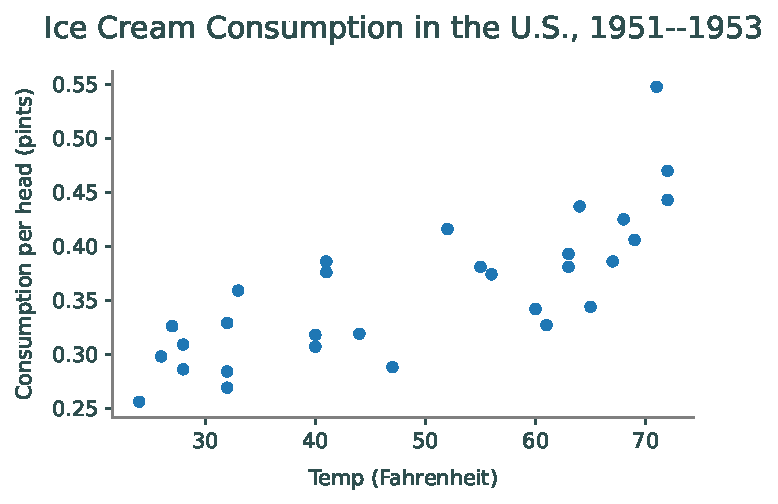
\includegraphics[width=.7\textwidth]{figures/ice_cream_good.pdf}
    \caption{Source:  Hildreth, C. and J. Lu (1960) \emph{Demand relations with autocorrelated disturbances}, Technical Bulletin No 2765, Michigan State University.}
    \label{fig:labels}
\end{figure}

\begin{warn}
Visualizing data can inherit many biases of the visualizer and as a result can be intentionally misleading.
Examples of this include, but are not limited to, visualizing subsets of data that do not represent the whole of the data and having purposely misconstrued axes.
Every data visualizer has the responsibility to avoid including biases in their visualizations to ensure data is being represented informatively and accurately.
\end{warn}
% Problem 4
\begin{problem}
The dataset \li{college.csv} contains information from 1995 on universities in the United States.
To access information on variable names, go to \url{https://cran.r-project.org/web/packages/ISLR/ISLR.pdf}.
Create 3 plots that compare variables or universities.
These plots should answer questions about the data, e.g. what is the distribution of graduation rates or do schools with lower student to faculty ratios have higher tuition costs.
These three plots should be easy to understand and have clear variable names and citations.
\end{problem}

\begin{comment}
\begin{problem}
The \li{pydataset} module contains numerous data sets, each stored as a pandas \li{DataFrame}.
Read data on road accident deaths in the United States using the data set \li{road} in the \li{pydataset} module.
Using this data, answer the following questions:

\begin{enumerate}
\item Does higher population density indicate higher fuel consumption?
\item Does a correlation exist between number of drivers and number of deaths in a state?
\item Does the temperature of a state in January affect its population density?
\end{enumerate}

Support each claim with a visualization and make sure the visualizations are clearly labeled and easy to understand.
Include any citations provided by the data set.

(Hint: Consider how outliers may be skewing the data.)
\end{problem}

% Problem 5
\begin{problem}
The file \li{new_york_crime_clean.csv} contains data on New York City crimes and felonies from 2000-2017 taken from \url{https://www1.nyc.gov/site/nypd/stats/crime-statistics/historical.page}.
Use this data to answer the following questions and give visualizations supporting each claim:
\begin{enumerate}
\item What are the most common and least common crimes?
\item Does a trend exist between robbery and drug felonies? If so, what is the trend?
\item Which crimes have had the largest distributions?
\end{enumerate}
Use a different style of visualization for each question.
Make sure that each plot is well labeled and contains citations.

(Hint: Use plt.axis('scaled') or plt.axis('square') to make sure x- and y-axis are the same.)
\end{problem}
\end{comment}
